\title{Experimental Laboratory 2\\Analysis of the velocity field in the wake of a circular cylinder}
\author{
        Sergio M. Vanegas A.\\
        Francesco de Pas\\
                Department of Mathematics\\
        Polimi---Politecnico di Milano\\
        Milano, Italia
}
\date{\today}

\documentclass[12pt]{article}

\usepackage{amsmath}
\usepackage{graphicx}
\usepackage{siunitx}

\begin{document}
\maketitle

\begin{abstract}

        The goal of this laboratory is to analyze the velocity field around a cylinder in a water channel flow, focusing on the wake region. Reference is made to experimental data obtained through the Particle Streak Velocimetry (PSV) technique, which essentially resides on seeding the flow with small particles and shoot a video of the light-sheet illumination plane. The camera has a high exposure time, intended as the time duration of a frame, so that each particle leaves a streak on the image, as exemplified in Figure~\ref{fig:camera} below. The images then are processed to get the velocity field. In the case study proposed, the Reynolds number of the cylinder \(\text{Re} = \frac{D U_\infty}{\nu}\) is within the range of the “sub-critical regime”; therefore, it will be not surprising to notice that the flow separates at a certain distance from the front stagnation point, causing a recirculation zone behind of it, and that a turbulent oscillating wake is created by the shedding of two counter-rotating vortexes.\cite{FL:05}

        \begin{figure}[ht!]
                \centering
                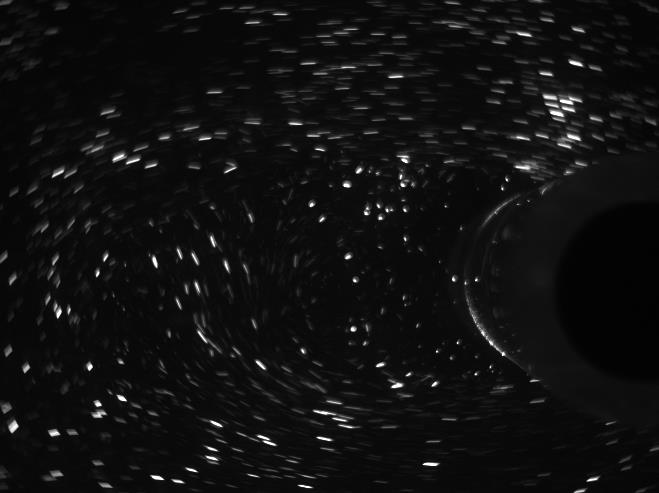
\includegraphics[width=\textwidth]{Camera_Acquisition.png}
                \caption{Exemplary image from the camera acquisition}
                \label{fig:camera}
        \end{figure}

        The scheme of the experiment is reported in the figure. The flow is from right to left in order to be consistent with the location of the PSV acquisition system in the water channel setup. The framing of the camera, which is the measurement field, is a vertical plane in the mid-section of the channel. The coordinate system of the PSV acquisition is $ (X,Y) $, as reported in Figure~\ref{fig:sketch}.

        \begin{figure}[ht!]
                \centering
                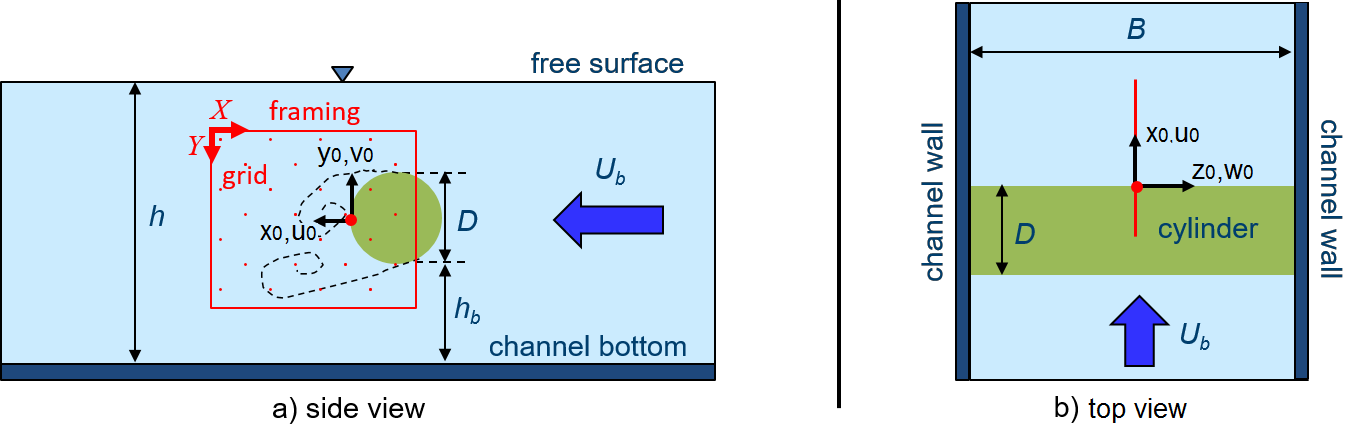
\includegraphics[width=\textwidth]{Sketch.png}
                \caption{Sketch of the experiment with the PSV frame and the two coordinate systems}
                \label{fig:sketch}
        \end{figure}

\end{abstract}

\section{Introduction}

        The input data of the problem are summarized in Table~\ref{tab:parameters}.

        \begin{table}[ht!]
                \centering
                \begin{tabular}{llll}
                        \hline
                        \textbf{Symbol} & \textbf{Parameter}    & \textbf{Value}        & \textbf{Units} \\ \hline
                        \textit{B}      & Width of the Channel  & $0.5$ & \textit{m} \\
                        \textit{D}      & Diameter of the Cylinder      & $0.06$        & \textit{m} \\
                        \textit{$f_s$}  & Sampling Frequency    & $50$  & \textit{Hz} \\
                        \textit{h}      & \begin{tabular}[c]{@{}l@{}}Water level in the channel\\upstream of the cylinder\end{tabular}  & $0.42$        & \textit{m} \\
                        \textit{$h_b$}  & \begin{tabular}[c]{@{}l@{}}Distance of the cylinder\\wall from the channel bottom\end{tabular}        & $0.18$        & \textit{m} \\
                        \textit{Q}      & Volumetric flow rate of water & $35$  & \textit{l/s} \\
                        \textit{res}    & Resolution of the images      & $3040$        & \textit{px/m} \\
                        \textit{$\rho$} & Density of water      & $998$ & \textit{$\text{kg}/m^3$} \\
                        \textit{$\mu$}  & Dynamic viscosity of water    & $0.001$       & \textit{$\text{Pa} \cdot s$} \\ \hline
                \end{tabular}
                \caption{Experimental settings - Input data}
                \label{tab:parameters}
        \end{table}

        For the post-processing of the PSV data, the frame was divided into a regular grid of 23x30 uniform cells along the directions X and Y, indicated in Figure~\ref{fig:sketch} (left). The number of time steps is 1499, and the duration of each of them is equal to \(1/f_s\), being $f_s$ the sampling frequency. The complete set of acquisition data is provided in the MATLAB workspace \textit{PSVdata.mat}, which includes the variables reported in Table~\ref{tab:image_data}.

        \begin{table}[ht!]
                \begin{tabular}{lll}
                        \hline
                        \textbf{Variable}       & \textbf{Type} & \textbf{Value} \\ \hline
                        \textit{Grid\_Xpx}      & 23x30 matrix  & \begin{tabular}[c]{@{}l@{}}X-coordinates of grid centers\\in the framing {[}in px{]}\end{tabular} \\
                        \textit{Grid\_Ypx}      & 23x30 matrix  & \begin{tabular}[c]{@{}l@{}}Y-coordinates of grid centers\\in the framing {[}in px{]}\end{tabular} \\
                        \textit{SXpx}   & 23x30x1499 matrix     & \begin{tabular}[c]{@{}l@{}}X displacement {[}in px{]}\\for every time step\end{tabular} \\
                        \textit{SYpx}   & 23x30x1499 matrix     & \begin{tabular}[c]{@{}l@{}}Y displacement {[}in px{]}\\for every time step\end{tabular} \\ \hline
                \end{tabular}
                \caption{Acquisition Data - Parameters}
                \label{tab:image_data}
        \end{table}

        A static snapshot of the PSV frame with a ruler close to the cylinder has been taken before running the experiment, and it is provided as an image file (\textit{ref\_image.png}). A small preview of the image file is reported below in Figure~\ref{fig:reference}. The scope of this preliminary step is two-fold. On the one hand, it has been used to estimate the resolution of the image as \( \text{res} = 3040 \text{px/cm} \), which is here already given as input for the sake of simplicity. On the other hand, it is used to turn the “pixel-based” matrixes \textit{Grid\_Xpx}, \textit{Grid\_Ypx}, \textit{SXpx}, and \textit{Sypx} into the corresponding dimensional matrixes in the new coordinate system (x0, y0), centered in the rear stagnation point and directed, as shown in Figure~\ref{fig:sketch} (left).

        \begin{figure}[ht!]
                \centering
                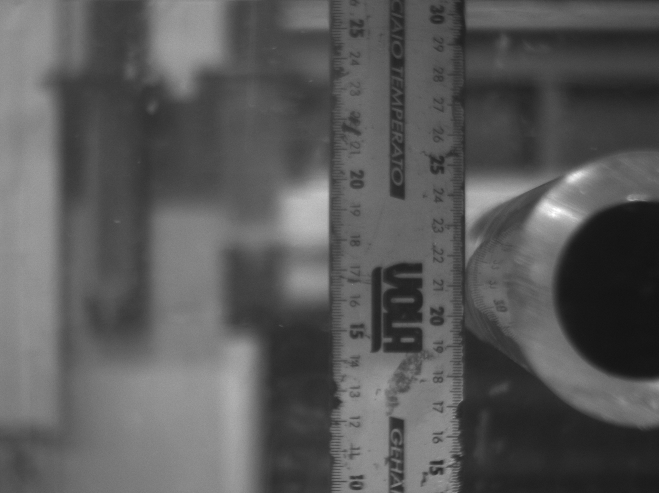
\includegraphics[width=\textwidth]{Reference.png}
                \caption{Reference image}
                \label{fig:reference}
        \end{figure}

        The remainder of the report is organized as follows: in Section~\ref{sec:bulk_velocity}, we approximate the channel Bulk velocity, which will be fundamental for the analysis of the experimental data; in Section~\ref{sec:dimensional}, we transform the pixel-based data inside the MATLAB file in order to adjust the axis and variables to real-world units of measurement; in Section~\ref{sec:RANS}, we calculate the Reynolds-average velocity field from the transformed data; in Section~\ref{sec:dynamics}, we investigate the dynamic evolution of the flow both in the time and frequency domains; finally, in Section~\ref{sec:spectra} we discuss the point-based spectra of the individual velocity fields.

        For the animated view of the experimental data, refer to the attached script.

\section{Bulk Velocity Approximation} \label{sec:bulk_velocity}

        Since the experiments involve a water flow in a finite size channel, $ U_b \neq U_\infty $; nevertheless, it is a reasonable first approximation for our case of study. We approximate the channel bulk velocity through the expression in Equation~\ref{eq:Ub}. Then, we use this value to approximate the Reynolds number as in Equation~\ref{eq:Re}.

        \begin{equation} \label{eq:Ub}
                U_b = \frac{Q}{B h} = \SI{1.667E-1}{\metre \per \second}
        \end{equation}

        \begin{equation} \label{eq:Re}
                \text{Re} = \frac{D U_\infty}{\nu} \approx \frac{D U_b}{\nu} = \num{9.980E3}
        \end{equation}

\section{Data dimensional treatment} \label{sec:dimensional}

        In order to apply the necessary transformations, we performed a pixel-count on the reference image (Figure~\ref{fig:reference}) using GIMP. We first located the domain half-point by measuring the cylinder height and cutting it in half, just like in Figure~\ref{fig:half_point}. Then, we measured the distance from the image origin to the physical origin (right side of the ruler, cylinder half-point) to get the pixel value of the new origin, as it is shown in Figure~\ref{fig:origin}.

        \begin{figure}[ht!]
                \centering
                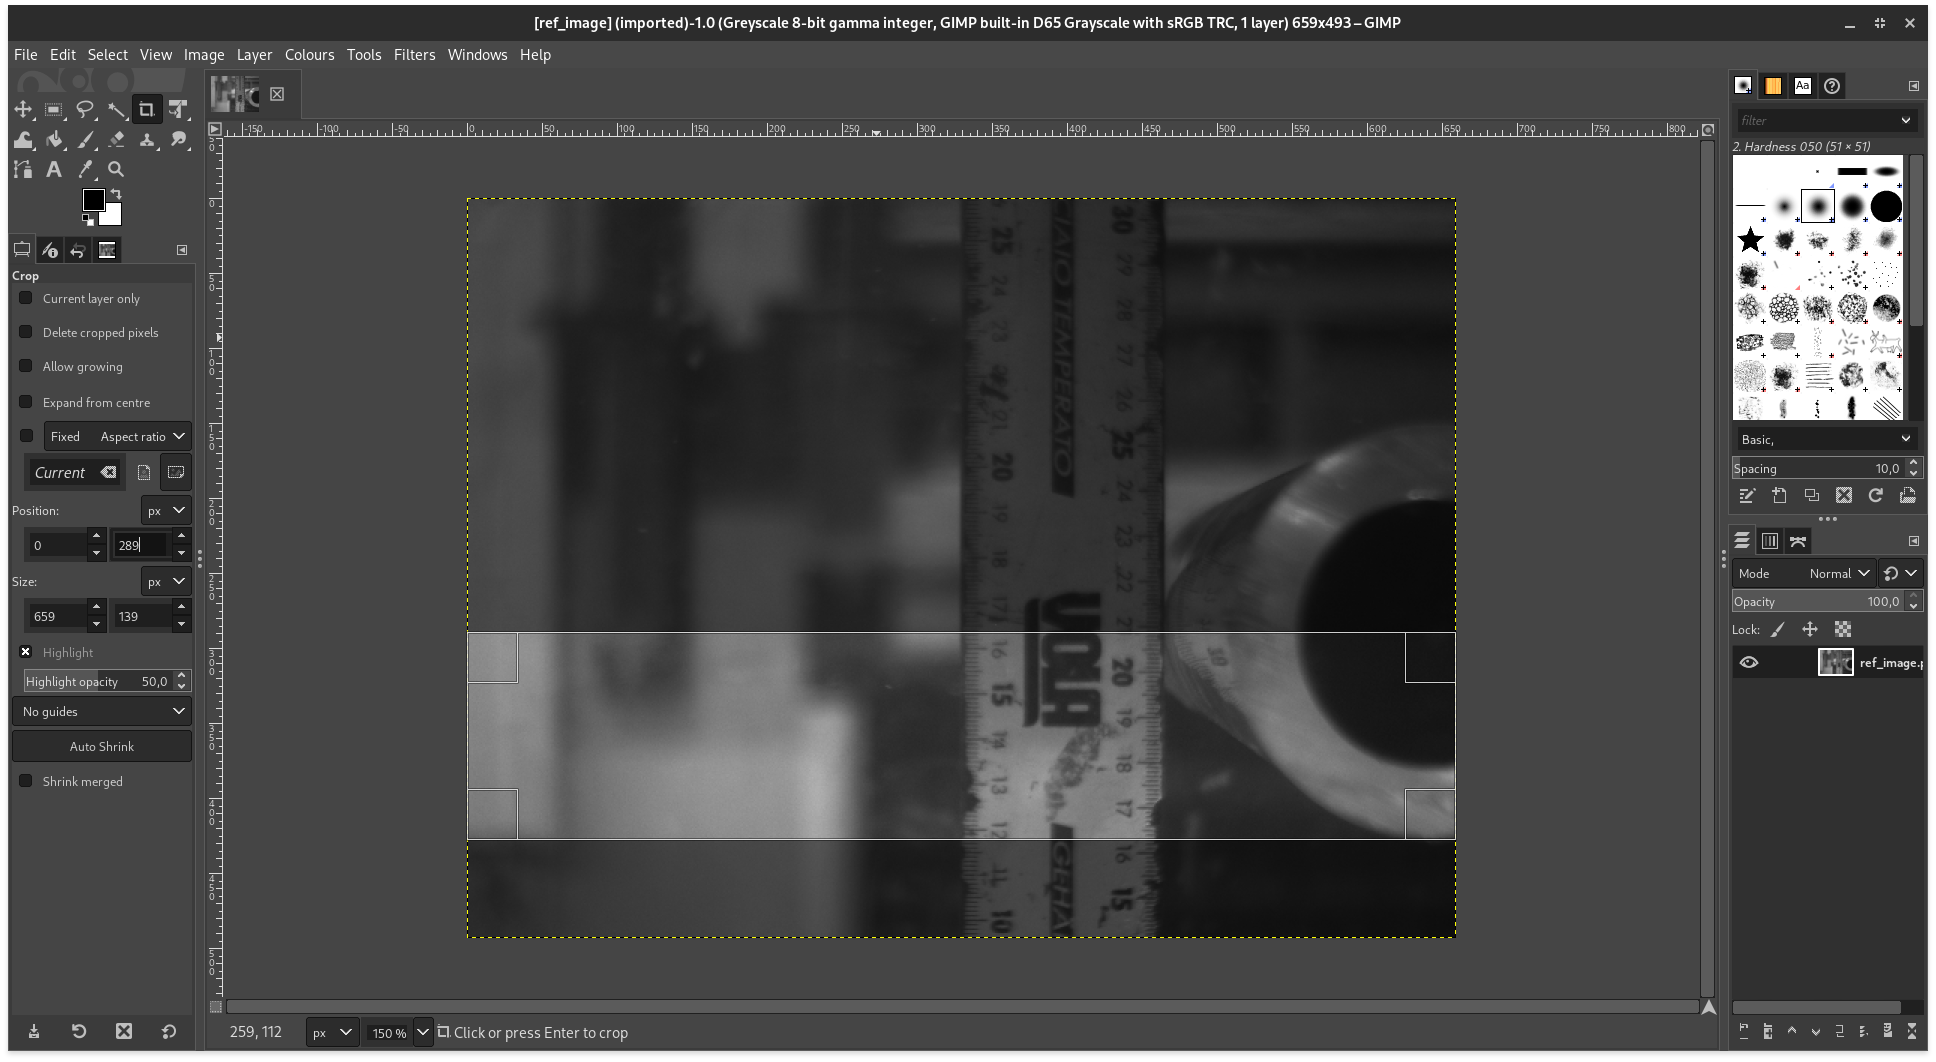
\includegraphics[width=\textwidth]{Half_Point_Finder.png}
                \caption{Location of the new vertical origin}
                \label{fig:half_point}
        \end{figure}

        \begin{figure}[ht!]
                \centering
                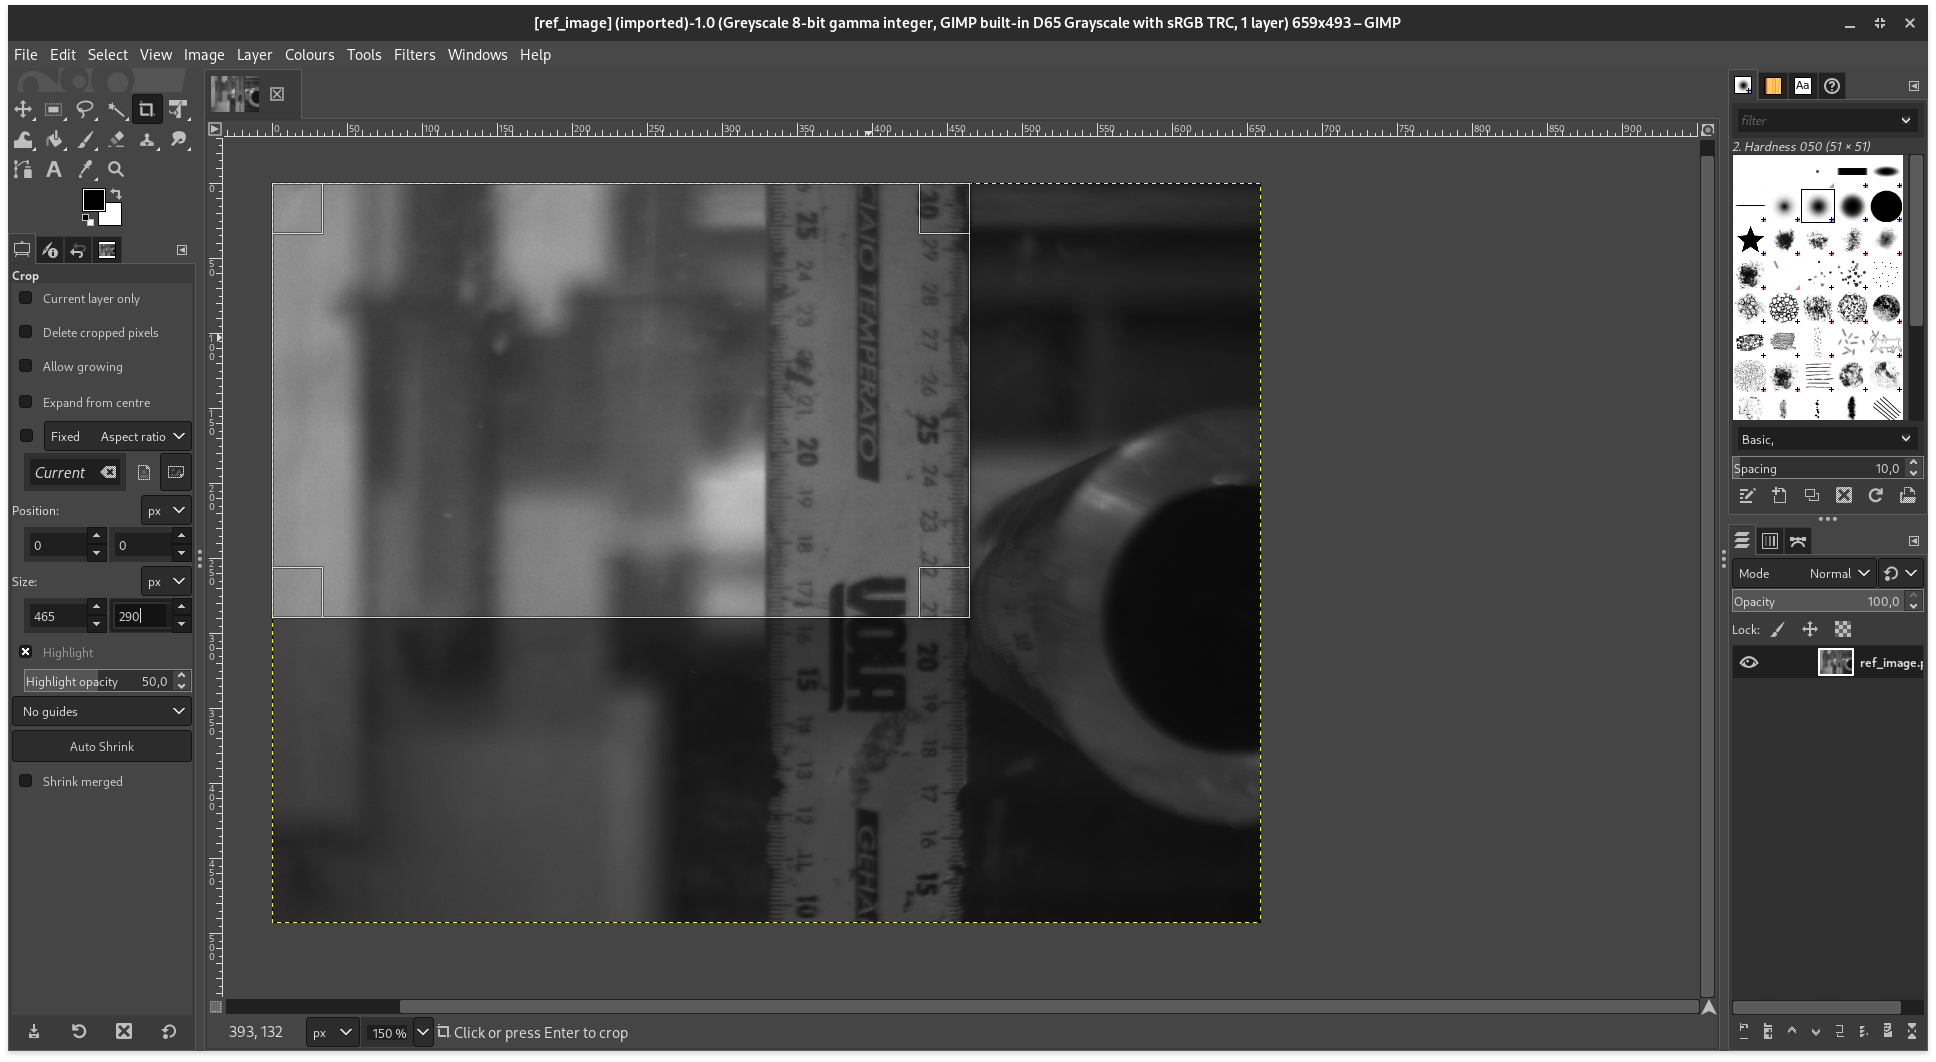
\includegraphics[width=\textwidth]{New_Reference.png}
                \caption{Location of the new physical origin}
                \label{fig:origin}
        \end{figure}

        Using these values, we proceeded to transform and normalize our grid and displacement data. As a result, we got the variables \textit{Grid\_x0\_D}, \textit{Grid\_y0\_D}, \textit{u0\_Ub} and \textit{v0\_Ub}.

\section{Reynolds-average velocity} \label{sec:RANS}

        Once the whole dataset had been processed for analysis, we proceeded to time-average the pointwise instantaneous velocity (both horizontal and vertical). With this, we plotted both the vector field and the interpolated streamlines in Figure~\ref{fig:vf} and Figure~\ref{fig:streamlines}; a circle representing the cylinder disturbing the flow was drawn in red on both figures for reference. We can see how part of the flow overlaps because of the camera perspective; nevertheless, the flow recirculation is coherent with the expected behaviour.

        \begin{figure}[ht!]
                \centering
                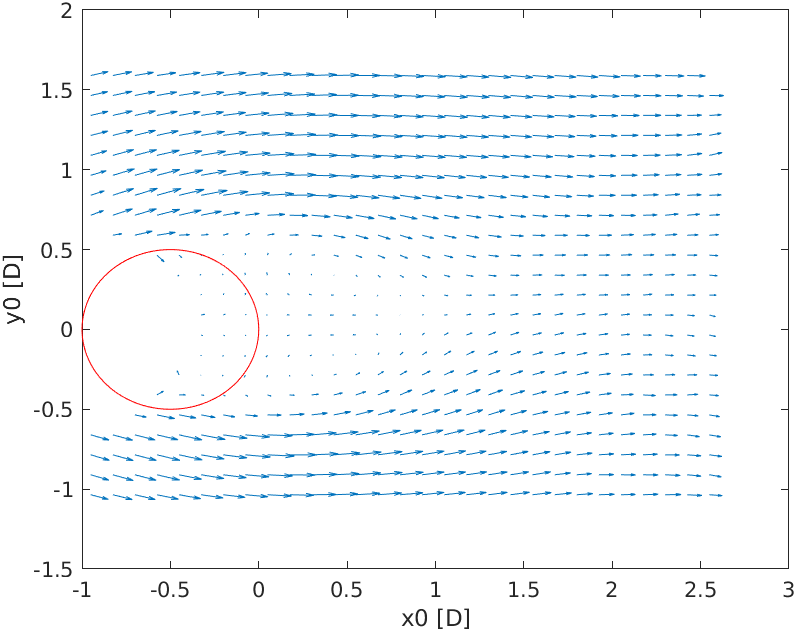
\includegraphics[width=\textwidth]{Vector_Field.png}
                \caption{Velocity vector field}
                \label{fig:vf}
        \end{figure}

        \begin{figure}[ht!]
                \centering
                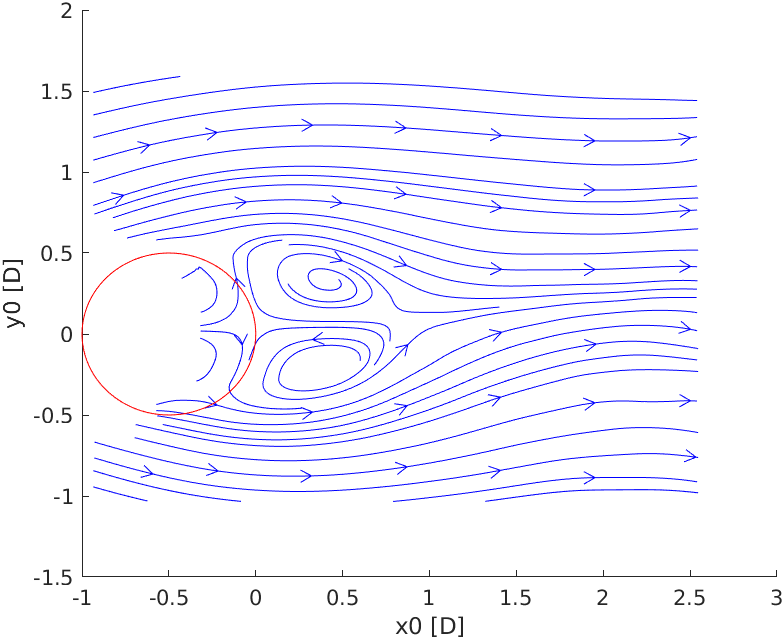
\includegraphics[width=\textwidth]{Streamlines.png}
                \caption{Flow streamlines}
                \label{fig:streamlines}
        \end{figure}

        Lastly, we plotted more specific profiles in Figure~\ref{fig:centerline_average} and Figure~\ref{fig:vertical_profiles} (velocity fields normalized w.r.t. Channel Bulk Velocity).

        \begin{figure}[ht!]
                \centering
                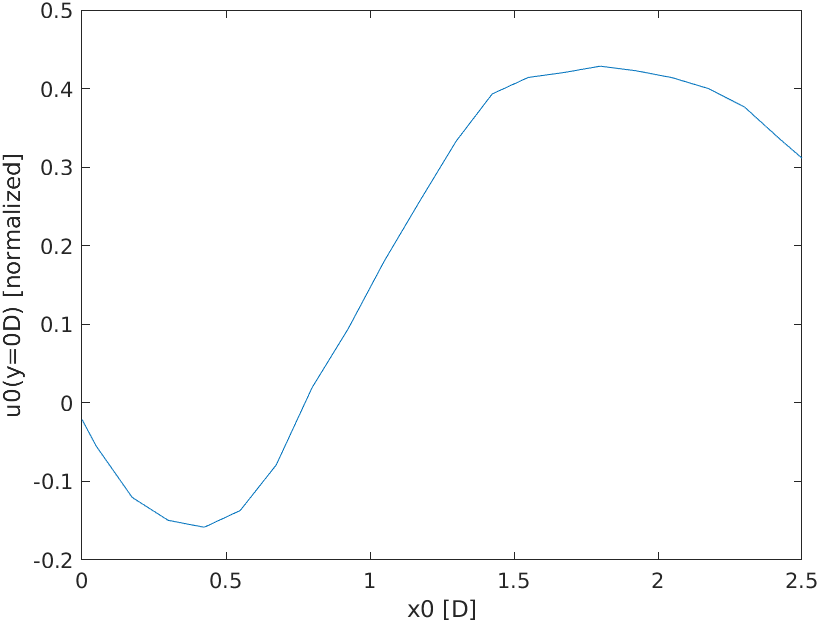
\includegraphics[width=\textwidth]{Centerline_Profile.png}
                \caption{Horizontal velocity centerline profile}
                \label{fig:centerline_average}
        \end{figure}

        \begin{figure}[ht!]
                \centering
                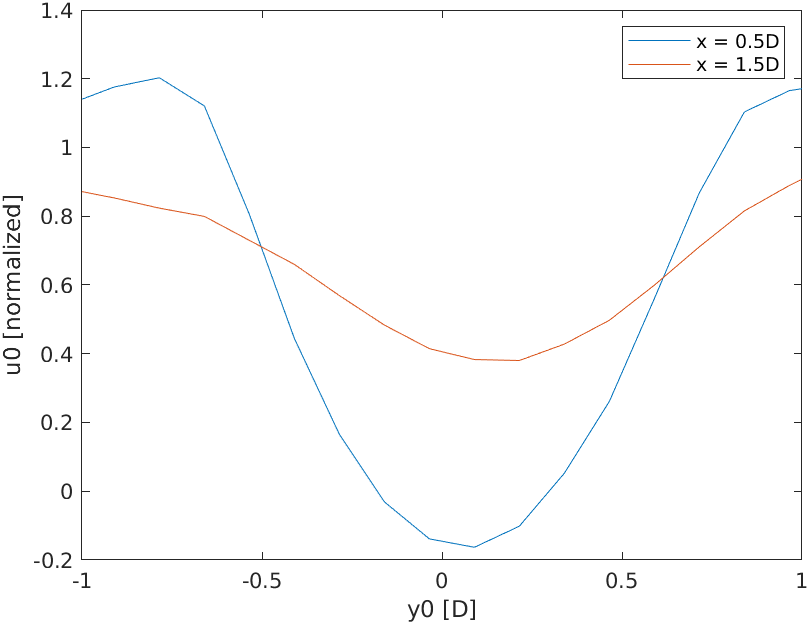
\includegraphics[width=\textwidth]{Vertical_Profiles.png}
                \caption{Horizontal velocity vertical profiles}
                \label{fig:vertical_profiles}
        \end{figure}

\section{Flow Dynamic Evolution} \label{sec:dynamics}

        In order to investigate the Flow's dynamic evolution, we performed a pointwise moving average over the instantaneous velocity data as a pre-processing procedure to remove high-frequency signal error.

        We then plotted the time history of the normalized vertical velocity in the closest (positive) point to the origin (w.r.t. the processed cartesian coordinates) available in the data array, which can be observed in Figure~\ref{fig:origin_history}.

        \begin{figure}[ht!]
                \centering
                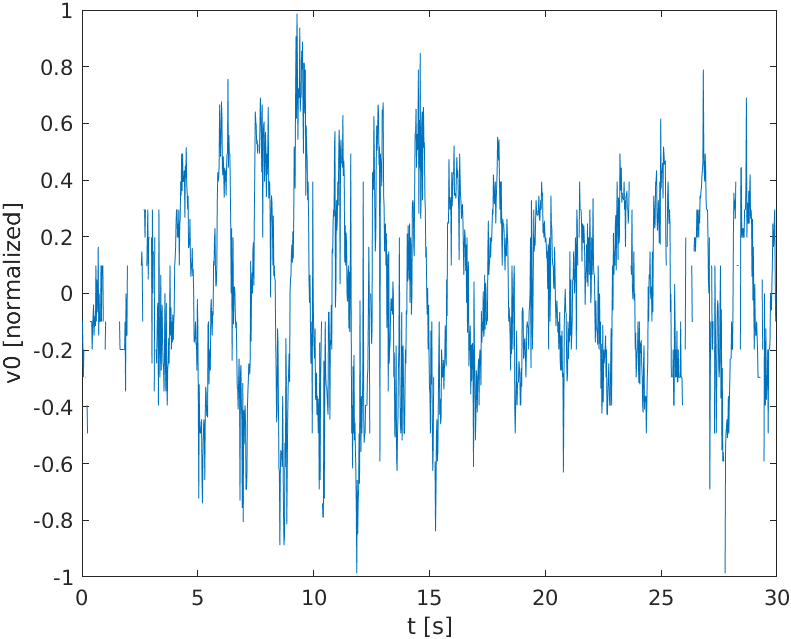
\includegraphics[width=\textwidth]{history.png}
                \caption{Approximate history of the normalized vertical velocity at the origin}
                \label{fig:origin_history}
        \end{figure}

        Since not a lot of information can be extracted from the time profile, we then calculated the FFT of the aforementioned signal in order to extract the vortex shedding frequency $ f $ of the velocity field. As it can be observed in Figure~\ref{fig:fft_single}, $ f \approx \SI{5.67423E-1}{\hertz} $.

        \begin{figure}[ht!]
                \centering
                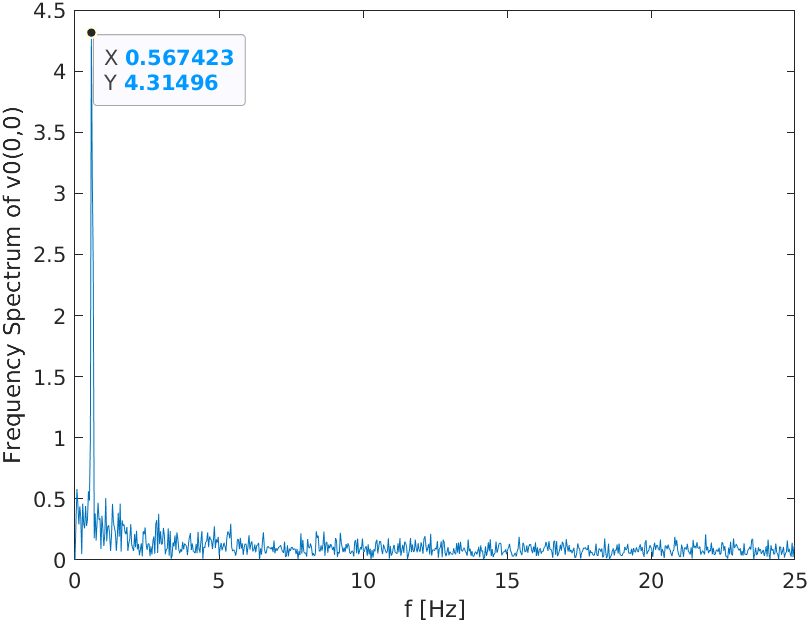
\includegraphics[width=\textwidth]{FFT_single.png}
                \caption{Approximate frequency spectrum of the normalized vertical velocity at the origin}
                \label{fig:fft_single}
        \end{figure}

        In order to corroborate this result, we calculated the Strouhal number $ \text{SR} = \frac{f U_b}{D} = 0.2043 $ and tested this value against the expected Reynolds number presented in Figure~\ref{fig:strouhal}, which is approximately ten thousand. As a consequence, we can validate the frequency analysis of the experiment.

        \begin{figure}[ht!]
                \centering
                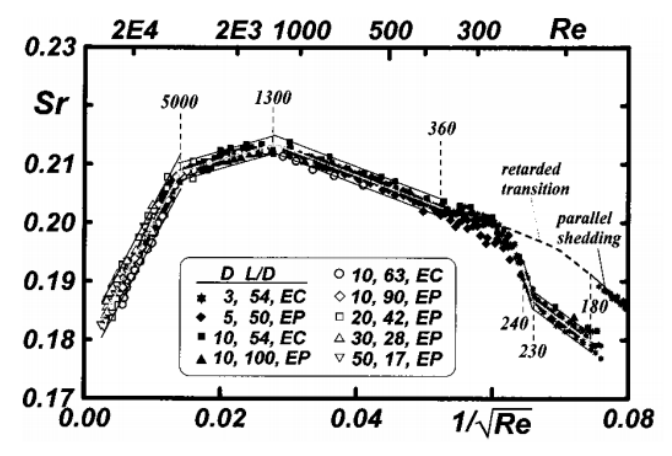
\includegraphics[width=\textwidth]{Strouhal.png}
                \caption{Strouhal number versus Reynolds number for unbounded flow over a circular cylinder \cite{doi:10.1063/1.869675}}
                \label{fig:strouhal}
        \end{figure}

\section{Frequency Spectra Analysis} \label{sec:spectra}

        Finally, we overlapped all pointwise frequency spectrum of the normalized vertical velocity. Even if these profiles changed consistently from point to point, the fundamental frequency and overall shape of the magnitude of the each spectrum remained unchanged throughout the data array, proving that the shedding frequency characterizes not only a coordinate of the domain, but the flow itself.

\newpage

\bibliographystyle{abbrv}
\bibliography{main}

\end{document}
